\documentclass[12pt, a4paper, twocolumn]{article}
\usepackage{lmodern}
\usepackage{amssymb,amsmath}
\usepackage{ifxetex,ifluatex}
\usepackage{fixltx2e} % provides \textsubscript
\ifnum 0\ifxetex 1\fi\ifluatex 1\fi=0 % if pdftex
  \usepackage[T1]{fontenc}
  \usepackage[utf8]{inputenc}
\else % if luatex or xelatex
  \ifxetex
    \usepackage{mathspec}
  \else
    \usepackage{fontspec}
  \fi
  \defaultfontfeatures{Ligatures=TeX,Scale=MatchLowercase}
\fi
% use upquote if available, for straight quotes in verbatim environments
\IfFileExists{upquote.sty}{\usepackage{upquote}}{}
% use microtype if available
\IfFileExists{microtype.sty}{%
\usepackage[]{microtype}
\UseMicrotypeSet[protrusion]{basicmath} % disable protrusion for tt fonts
}{}
\PassOptionsToPackage{hyphens}{url} % url is loaded by hyperref
\usepackage[unicode=true]{hyperref}
\hypersetup{
            pdfborder={0 0 0},
            breaklinks=true}
\urlstyle{same}  % don't use monospace font for urls
\usepackage{color}
\usepackage{fancyvrb}
\newcommand{\VerbBar}{|}
\newcommand{\VERB}{\Verb[commandchars=\\\{\}]}
\DefineVerbatimEnvironment{Highlighting}{Verbatim}{commandchars=\\\{\}}
% Add ',fontsize=\small' for more characters per line
\newenvironment{Shaded}{}{}
\newcommand{\KeywordTok}[1]{\textcolor[rgb]{0.00,0.44,0.13}{\textbf{#1}}}
\newcommand{\DataTypeTok}[1]{\textcolor[rgb]{0.56,0.13,0.00}{#1}}
\newcommand{\DecValTok}[1]{\textcolor[rgb]{0.25,0.63,0.44}{#1}}
\newcommand{\BaseNTok}[1]{\textcolor[rgb]{0.25,0.63,0.44}{#1}}
\newcommand{\FloatTok}[1]{\textcolor[rgb]{0.25,0.63,0.44}{#1}}
\newcommand{\ConstantTok}[1]{\textcolor[rgb]{0.53,0.00,0.00}{#1}}
\newcommand{\CharTok}[1]{\textcolor[rgb]{0.25,0.44,0.63}{#1}}
\newcommand{\SpecialCharTok}[1]{\textcolor[rgb]{0.25,0.44,0.63}{#1}}
\newcommand{\StringTok}[1]{\textcolor[rgb]{0.25,0.44,0.63}{#1}}
\newcommand{\VerbatimStringTok}[1]{\textcolor[rgb]{0.25,0.44,0.63}{#1}}
\newcommand{\SpecialStringTok}[1]{\textcolor[rgb]{0.73,0.40,0.53}{#1}}
\newcommand{\ImportTok}[1]{#1}
\newcommand{\CommentTok}[1]{\textcolor[rgb]{0.38,0.63,0.69}{\textit{#1}}}
\newcommand{\DocumentationTok}[1]{\textcolor[rgb]{0.73,0.13,0.13}{\textit{#1}}}
\newcommand{\AnnotationTok}[1]{\textcolor[rgb]{0.38,0.63,0.69}{\textbf{\textit{#1}}}}
\newcommand{\CommentVarTok}[1]{\textcolor[rgb]{0.38,0.63,0.69}{\textbf{\textit{#1}}}}
\newcommand{\OtherTok}[1]{\textcolor[rgb]{0.00,0.44,0.13}{#1}}
\newcommand{\FunctionTok}[1]{\textcolor[rgb]{0.02,0.16,0.49}{#1}}
\newcommand{\VariableTok}[1]{\textcolor[rgb]{0.10,0.09,0.49}{#1}}
\newcommand{\ControlFlowTok}[1]{\textcolor[rgb]{0.00,0.44,0.13}{\textbf{#1}}}
\newcommand{\OperatorTok}[1]{\textcolor[rgb]{0.40,0.40,0.40}{#1}}
\newcommand{\BuiltInTok}[1]{#1}
\newcommand{\ExtensionTok}[1]{#1}
\newcommand{\PreprocessorTok}[1]{\textcolor[rgb]{0.74,0.48,0.00}{#1}}
\newcommand{\AttributeTok}[1]{\textcolor[rgb]{0.49,0.56,0.16}{#1}}
\newcommand{\RegionMarkerTok}[1]{#1}
\newcommand{\InformationTok}[1]{\textcolor[rgb]{0.38,0.63,0.69}{\textbf{\textit{#1}}}}
\newcommand{\WarningTok}[1]{\textcolor[rgb]{0.38,0.63,0.69}{\textbf{\textit{#1}}}}
\newcommand{\AlertTok}[1]{\textcolor[rgb]{1.00,0.00,0.00}{\textbf{#1}}}
\newcommand{\ErrorTok}[1]{\textcolor[rgb]{1.00,0.00,0.00}{\textbf{#1}}}
\newcommand{\NormalTok}[1]{#1}
\usepackage{longtable,booktabs}
% Fix footnotes in tables (requires footnote package)
\IfFileExists{footnote.sty}{\usepackage{footnote}\makesavenoteenv{long table}}{}
\usepackage{graphicx,grffile}
\makeatletter
\def\maxwidth{\ifdim\Gin@nat@width>\linewidth\linewidth\else\Gin@nat@width\fi}
\def\maxheight{\ifdim\Gin@nat@height>\textheight\textheight\else\Gin@nat@height\fi}
\makeatother
% Scale images if necessary, so that they will not overflow the page
% margins by default, and it is still possible to overwrite the defaults
% using explicit options in \includegraphics[width, height, ...]{}
\setkeys{Gin}{width=\maxwidth,height=\maxheight,keepaspectratio}
\IfFileExists{parskip.sty}{%
\usepackage{parskip}
}{% else
\setlength{\parindent}{0pt}
\setlength{\parskip}{6pt plus 2pt minus 1pt}
}
\setlength{\emergencystretch}{3em}  % prevent overfull lines
\providecommand{\tightlist}{%
  \setlength{\itemsep}{0pt}\setlength{\parskip}{0pt}}
\setcounter{secnumdepth}{0}
% Redefines (sub)paragraphs to behave more like sections
\ifx\paragraph\undefined\else
\let\oldparagraph\paragraph
\renewcommand{\paragraph}[1]{\oldparagraph{#1}\mbox{}}
\fi
\ifx\subparagraph\undefined\else
\let\oldsubparagraph\subparagraph
\renewcommand{\subparagraph}[1]{\oldsubparagraph{#1}\mbox{}}
\fi

% set default figure placement to htbp
\makeatletter
\def\fps@figure{htbp}
\makeatother


\date{}

\begin{document}





\begin{center}

\begin{@twocolumnfalse}
{\Huge \textbf{INHA UNIVERSITY}}

{\Huge \textbf{\\* IN TASHKENT}}

{\Huge \textbf{\\ (SPRING 2020 -- SOC4020)}}

{\Huge \textbf{\\ MULTIMEDIA}} 

{\Huge \textbf{\\ COMPUTING}}

{\Huge \textbf{(Technical Report)}}


Submitted by

\begin{longtable}[]{@{}llll@{}}
\toprule
Name & Surname & ID & Group\tabularnewline
\midrule
\endhead
Rakhmatjon & Khasanov & U1610183 & 001\tabularnewline
\bottomrule
\end{longtable}

\includegraphics{meta/output_29_0.png}

\end{@twocolumnfalse}

{\Large  \textbf{Seamless Face Cloning Using Face Segmentation by Delaunay Triangulation}} 
\end{center}

\tableofcontents

\begin{center}
{Mentored by \\ Dr. Uddin Ahmed Minhaz}
\end{center}
\clearpage

\subsection{Abstract}\label{header-n424}

This project demonstrate a demo system for automatic facial replacement
in images and video . The program extracts faces using face recognition
software, and aligns each extracted face to a specific coordinate. This
library is built offline, once, and can be accessed efficiently during
face replacement. Our substitution algorithm has three major phases.
First, given an input image, all the faces present are detected, aligned
with the face library's coordinate scheme, and picked candidate face
images from the face library that are identical to the face of the user
in appearance and pose. Second, the code changes the candidate's
posture, lighting and color to suit the presence of those in the input
shot, and merges the results smoothly. The project's approach does not
require a 3D model, is fully automated, and achieves extremely probable
outcomes through a wide variety of skin tones, lighting conditions and
points of view. It is clear how this methodology can be used for a range
of applications like face de-identification and generating beautiful
group portraits from a collection of photos.

\subsection{Introduction}\label{header-n413}

Face Fusion corresponds to the image processing technique of the
automated merging of two or more separate faces into one object, and is
commonly employed in the fields of photo synthesis, anonymity, image
enhancement, and entertainment applications. For example, if we choose
to share any of the fascinating stuff on social networks, we can use a
facial synthesis technique that can be described as a combination of
facial features and information to alter looks appropriately without
privacy leaks. As another kind of face fusion, face swapping blends
sections of one person's face with sections of the other's face to
create a new face picture. For example, in the implementation of virtual
hairstyle rendering, the client's face region can be merged with the
hair areas of the model images to generate new pictures, such that
clients can digitally search their own figures with various hairstyles.
This paper focuses on the face-swap issue of virtual hairstyle and
dressing browsing applications.

\subsection{Approach and Results}\label{header-n393}

The approach used for this project is Face Segment Replacement using Delaunay Triangulation. For this, we need to follow the following steps:

\paragraph{Taking two images}\label{header-n438}

\begin{figure}
	\centering
	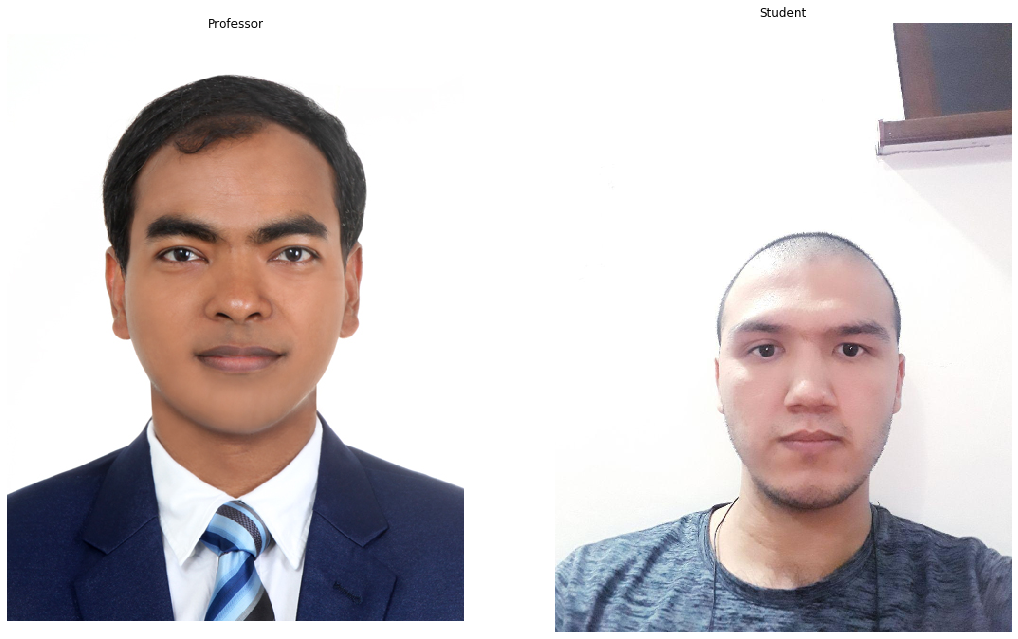
\includegraphics{meta/output_30_0.png}
	\caption{Taking two images}
\end{figure}

\begin{Shaded}
\small
\begin{Highlighting}[]
\NormalTok{img }\OperatorTok{=}\NormalTok{ cv2.imread(}\StringTok{"meta/professor.jpeg"}\NormalTok{)}
\NormalTok{img_gray }\OperatorTok{=}\NormalTok{ cv2.cvtColor(img, cv2.COLOR_BGR2GRAY)}

\NormalTok{img2 }\OperatorTok{=}\NormalTok{ cv2.imread(}\StringTok{"meta/student.jpg"}\NormalTok{)}
\NormalTok{img2_gray }\OperatorTok{=}\NormalTok{ cv2.cvtColor(img2,}\OperatorTok{\textbackslash{}}
\NormalTok{cv2.COLOR_BGR2GRAY)}
\end{Highlighting}
\end{Shaded}


\paragraph{Find landmark points of both images}\label{header-n150}

\begin{quote}
	We use the dlib library to identify facial landmarks.
	
	We use the dlib library to identify facial landmarks.\\
	I illustrate how to locate the key points in the code below.
	
	In this particular code that I'm displaying as an illustration that I
	detect the landmarks of the source image, you need to add it to the
	destination picture as well.
	
	You can download shape\emph{predictor}68\emph{face}landmarks.dat from
	the
	\href{https://github.com/AKSHAYUBHAT/TensorFace/blob/master/openface/models/dlib/shape_predictor_68_face_landmarks.dat}{link}
\end{quote}

\begin{Shaded}
\small
\begin{Highlighting}[]
\NormalTok{det}\OperatorTok{=}\NormalTok{ dlib.get_frontal_face_detector()}
\NormalTok{dat }\OperatorTok{=} \StringTok{"}\NormalTok{shape_predictor_-}\OperatorTok{}
\NormalTok{68_face_landmarks.dat}\StringTok{"}
\NormalTok{predictor }\OperatorTok{=}\NormalTok{ dlib.shape_predictor(dat)}

\NormalTok{faces }\OperatorTok{=}\NormalTok{ detector(img_gray)}
\ControlFlowTok{for}\NormalTok{ face }\KeywordTok{in}\NormalTok{ faces:}
\NormalTok{    landmarks }\OperatorTok{=}\NormalTok{ predictor(img_gray, face)}
\NormalTok{    landmarks_points }\OperatorTok{=}\NormalTok{ []}
\ControlFlowTok{for}\NormalTok{ n }\KeywordTok{in} \BuiltInTok{range}\NormalTok{(}\DecValTok{0}\NormalTok{, }\DecValTok{68}\NormalTok{):}
\NormalTok{        x }\OperatorTok{=}\NormalTok{ landmarks.part(n).x}
\NormalTok{        y }\OperatorTok{=}\NormalTok{ landmarks.part(n).y}
\NormalTok{        landmarks_points.append((x, y))}
\end{Highlighting}
\end{Shaded}

\begin{figure}
	\centering
	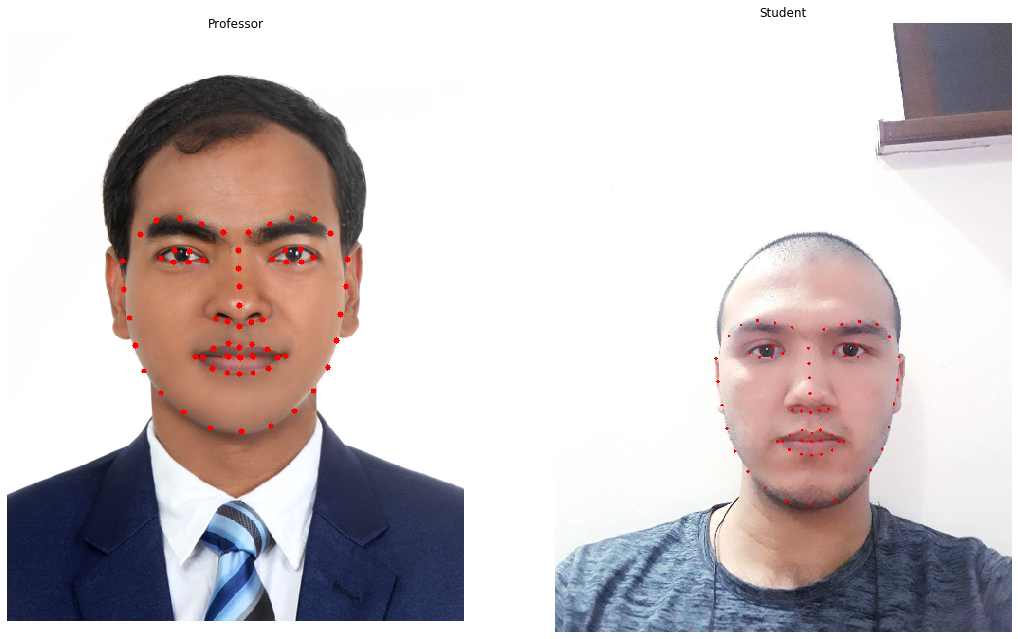
\includegraphics{meta/output_31_0.png}
	\caption{Find landmark points of both images}
\end{figure}

\paragraph{Delaunay triangulation of Source Image}\label{header-n153}

\begin{quote}
	And we segment the face into triangles. This phase is the center of our
	face swapping, as later we will simply interchange each triangle with
	the corresponding triangle of the destination picture.
	
	Why are we deviating the mask into triangles?\\
	We can't just take the face out of the source picture and place it in
	the destination picture because it's limited in scale and viewpoint.
	
	We can't adjust its scale and orientation right away, either, as the
	face will sacrifice its initial dimensions.\\
	Instead, if we divide the face into triangles, we would easily change
	each triangle to retain the proportions and suit the features of the new
	face, so, for example, whether you grin, close your eyes or open your
	mouth.
\end{quote}

\begin{Shaded}
\small
\begin{Highlighting}[]
\NormalTok{rect }\OperatorTok{=}\NormalTok{ cv2.boundingRect(convexhull)}
\NormalTok{subdiv }\OperatorTok{=}\NormalTok{ cv2.Subdiv2D(rect)}
\NormalTok{subdiv.insert(landmarks_points)}
\NormalTok{triangles }\OperatorTok{=}\NormalTok{ subdiv.getTriangleList()}
\NormalTok{triangles }\OperatorTok{=}\NormalTok{ np.array(triangles,}\OperatorTok{\textbackslash{}}
\NormalTok{ dtype}\OperatorTok{=}\NormalTok{np.int32)}
\end{Highlighting}
\end{Shaded}

\begin{figure}
	\centering
	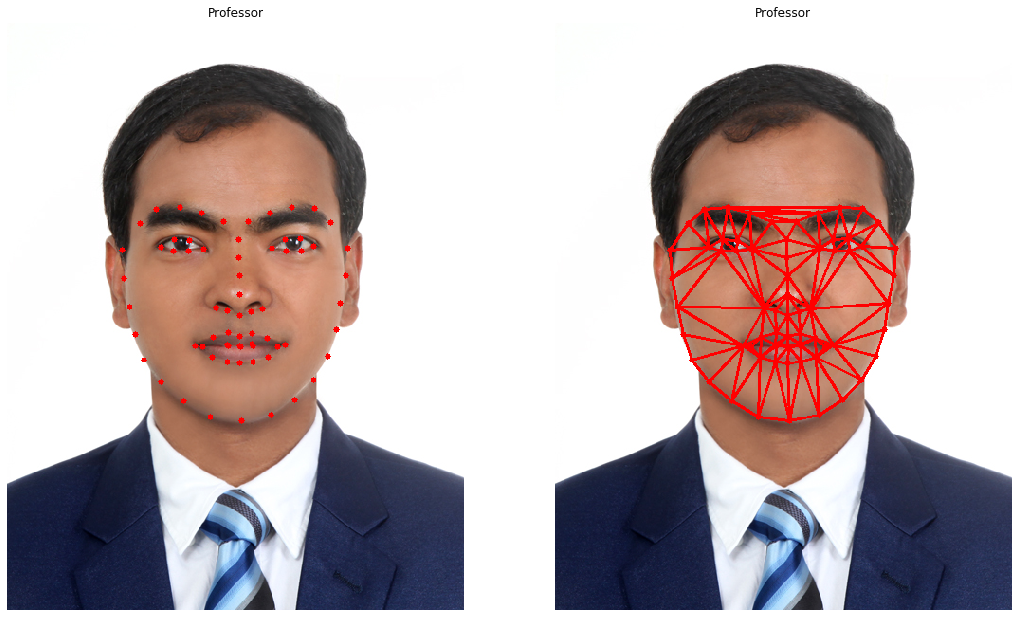
\includegraphics{meta/output_32_0.png}
	\caption{Delaunay triangulation of Source Image}
\end{figure}

\paragraph{Delaunay triangulation of Destination
	Image}\label{header-n156}

\begin{quote}
	The triangulation of the destination image has to provide the same
	patterns of the source picture triangulation.\\
	This implies that the relation of the points must be the same.
	
	So, after we do the triangulation of the source image, we take the
	indexes of the landmark points from that triangulation, so that we can
	replicate the same triangulation on the destination image.
\end{quote}

\begin{Shaded}
\small
\begin{Highlighting}[]
\NormalTok{indexes_triangles }\OperatorTok{=}\NormalTok{ []}
\ControlFlowTok{for}\NormalTok{ t }\KeywordTok{in}\NormalTok{ triangles:}
\NormalTok{    pt1 }\OperatorTok{=}\NormalTok{ (t[}\DecValTok{0}\NormalTok{], t[}\DecValTok{1}\NormalTok{])}
\NormalTok{    pt2 }\OperatorTok{=}\NormalTok{ (t[}\DecValTok{2}\NormalTok{], t[}\DecValTok{3}\NormalTok{])}
\NormalTok{    pt3 }\OperatorTok{=}\NormalTok{ (t[}\DecValTok{4}\NormalTok{], t[}\DecValTok{5}\NormalTok{])}\OperatorTok{}
\NormalTok{}
\NormalTok{    index_pt1 }\OperatorTok{=}\NormalTok{ np.where((points }\OperatorTok{==}\OperatorTok{\textbackslash{}}
\NormalTok{}\NormalTok{ pt1).}\BuiltInTok{all}\NormalTok{(axis}\OperatorTok{=}\DecValTok{1}\NormalTok{))}
\NormalTok{    index_pt1 }\OperatorTok{=}\NormalTok{ extract_index_nparray(index_pt1)}
\NormalTok{    index_pt2 }\OperatorTok{=}\NormalTok{ np.where((points }\OperatorTok{==}\OperatorTok{\textbackslash{}}
\NormalTok{}\NormalTok{ pt2).}\BuiltInTok{all}\NormalTok{(axis}\OperatorTok{=}\DecValTok{1}\NormalTok{))}
\NormalTok{    index_pt2 }\OperatorTok{=}\NormalTok{ extract_index_nparray(index_pt2)}
\NormalTok{    index_pt3 }\OperatorTok{=}\NormalTok{ np.where((points }\OperatorTok{==}\OperatorTok{\textbackslash{}}
\NormalTok{}\NormalTok{ pt3).}\BuiltInTok{all}\NormalTok{(axis}\OperatorTok{=}\DecValTok{1}\NormalTok{))}
\NormalTok{    index_pt3 }\OperatorTok{=}\NormalTok{ extract_index_nparray(index_pt3)}
\ControlFlowTok{if}\NormalTok{ index_pt1 }\KeywordTok{is} \KeywordTok{not} \VariableTok{None} \KeywordTok{and}\NormalTok{ index_pt2 }\KeywordTok{is} \KeywordTok{not} \VariableTok{None} \OperatorTok{\textbackslash{}}
\KeywordTok{and}\NormalTok{ index_pt3 }\KeywordTok{is} \KeywordTok{not} \VariableTok{None}\NormalTok{:}
\NormalTok{        triangle }\OperatorTok{=}\NormalTok{ [index_pt1, index_pt2,}\OperatorTok{\textbackslash{}}
\NormalTok{ index_pt3]}
\NormalTok{        indexes_triangles.append(triangle)}
\end{Highlighting}
\end{Shaded}

\begin{quote}
	If we have the index triangles, we loop around them and triangulate the
	destination nose.
\end{quote}

\begin{Shaded}
\small
\begin{Highlighting}[]
\ControlFlowTok{for}\NormalTok{ triangle_index }\KeywordTok{in}\NormalTok{ indexes_triangles:}
\NormalTok{    tr1_pt1 }\OperatorTok{=}\NormalTok{ landmarks_points2[triangle_index[}\DecValTok{0}\NormalTok{]]}
\NormalTok{    tr1_pt2 }\OperatorTok{=}\NormalTok{ landmarks_points2[triangle_index[}\DecValTok{1}\NormalTok{]]}
\NormalTok{    tr1_pt3 }\OperatorTok{=}\NormalTok{ landmarks_points2[triangle_index[}\DecValTok{2}\NormalTok{]]}
\NormalTok{    triangle2 }\OperatorTok{=}\NormalTok{ np.array([tr1_pt1, tr1_pt2, }\OperatorTok{\textbackslash{}}
\NormalTok{                          tr1_pt3], np.int32)}
\end{Highlighting}
\end{Shaded}

\begin{figure}
	\centering
	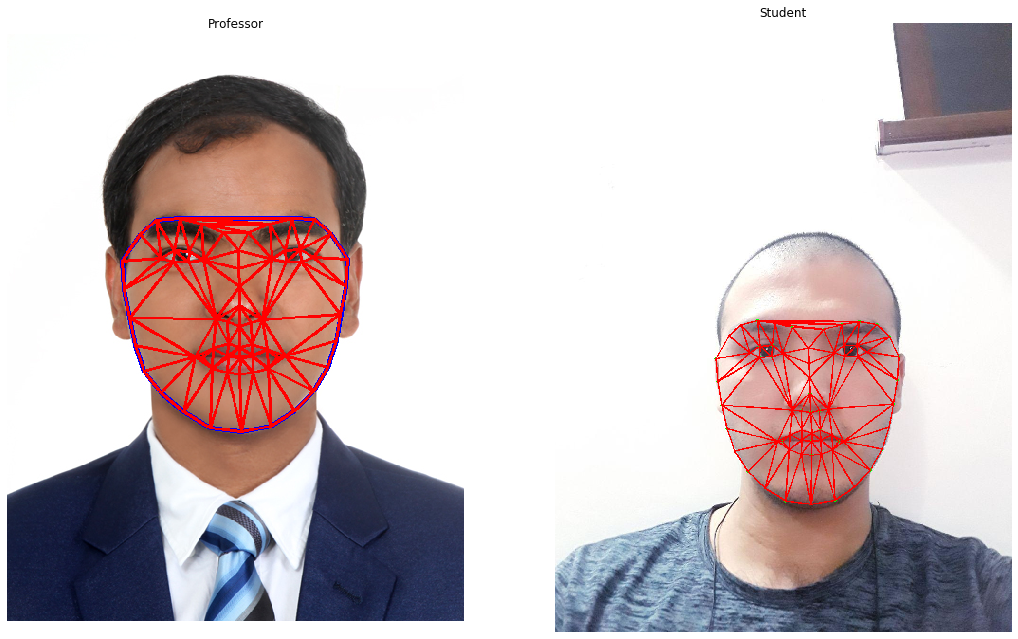
\includegraphics{meta/output_34_0.png}
	\caption{Delaunay triangulation of Destination Image}
\end{figure}

\paragraph{Extract and warp triangles}\label{header-n160}

\begin{quote}
	When we have the triangulation of both images, we take the root face
	triangles and remove them.\\
	We also need to take the coordinates of the destination face triangles
	so that we can warp the source face triangles to the same size and
	perspective of the matchin triangle on the destination face.
\end{quote}

\begin{Shaded}
\small
\begin{Highlighting}[]
\NormalTok{points }\OperatorTok{=}\NormalTok{ np.float32(points)}
\NormalTok{points2 }\OperatorTok{=}\NormalTok{ np.float32(points2)}
\NormalTok{M }\OperatorTok{=}\NormalTok{ cv2.getAffineTransform}\OperatorTok{\textbackslash{}}
\NormalTok{(points, points2)}
\NormalTok{warped_triangle }\OperatorTok{=}\NormalTok{ cv2.warpAffine}\OperatorTok{\textbackslash{}}
\NormalTok{(cropped_triangle, M, (w, h))}
\NormalTok{warped_triangle }\OperatorTok{=}\NormalTok{ cv2.bitwise_and}\OperatorTok{\textbackslash{}}
\NormalTok{(warped_triangle, warped_triangle, }\OperatorTok{\textbackslash{}}
\NormalTok{mask}\OperatorTok{=}\NormalTok{cropped_tr2_mask)}
\end{Highlighting}
\end{Shaded}

\begin{figure}
	\centering
	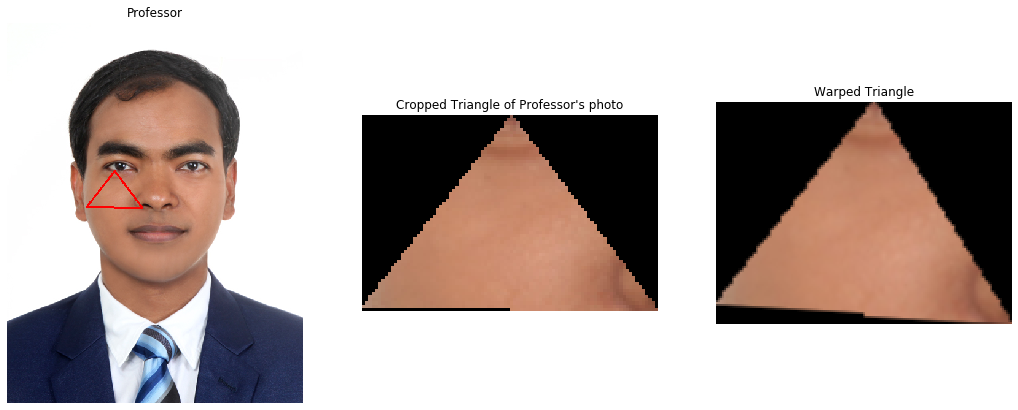
\includegraphics{meta/output_35_0.png}
	\caption{Extract and warp triangles}
\end{figure}

\paragraph{Link the warped triangles together}\label{header-n228}

\begin{quote}
	Once we've cut and twisted all the triangles we need to link them
	together.\\
	We 're only restoring the face using the triangulation template, with
	the only exception being this time we 're bringing the twisted triangle
	back.\\
	The mask is able to be substituted at the conclusion of this service.
\end{quote}

\begin{Shaded}
\small
\begin{Highlighting}[]
\NormalTok{img2_new_face }\OperatorTok{=}\OperatorTok{\textbackslash{}}
\NormalTok{}\NormalTok{ np.zeros((}\DecValTok{1155}\NormalTok{, }\DecValTok{849}\NormalTok{, }\DecValTok{3}\NormalTok{), np.uint8)}
\NormalTok{img2_new_face_rect_area }\OperatorTok{=}\OperatorTok{\textbackslash{}}
\NormalTok{}\NormalTok{ img2_new_face[y: y }\OperatorTok{+}\NormalTok{ h, x: x }\OperatorTok{+}\NormalTok{ w]}
\NormalTok{img2_new_face_rect_area_gray }\OperatorTok{=}\OperatorTok{\textbackslash{}}
\NormalTok{}\NormalTok{ cv2.cvtColor(img2_new_face_rect_area, }\OperatorTok{\textbackslash{}}
\NormalTok{cv2.COLOR_BGR2GRAY)}
\NormalTok{_, mask_triangles_designed }\OperatorTok{=}\OperatorTok{\textbackslash{}}
\NormalTok{cv2.threshold(img2_new_face_rect_area_gray,}\OperatorTok{\textbackslash{}}
\DecValTok{1}\NormalTok{, }\DecValTok{255}\NormalTok{, cv2.THRESH_BINARY_INV)}
\NormalTok{warped_triangle }\OperatorTok{=}\NormalTok{ cv2.bitwise_and}\OperatorTok{\textbackslash{}}
\NormalTok{(warped_triangle, warped_triangle, }\OperatorTok{\textbackslash{}}
\NormalTok{mask}\OperatorTok{=}\NormalTok{mask_triangles_designed)}
\NormalTok{img2_new_face_rect_area }\OperatorTok{=}\OperatorTok{\textbackslash{}}
\NormalTok{cv2.add(img2_new_face_rect_area, warped_triangle)}
\NormalTok{img2_new_face[y: y }\OperatorTok{+}\NormalTok{ h, x: x }\OperatorTok{+}\NormalTok{ w] }\OperatorTok{=}\OperatorTok{\textbackslash{}}
\NormalTok{img2_new_face_rect_area}
\end{Highlighting}
\end{Shaded}

\begin{figure}
	\centering
	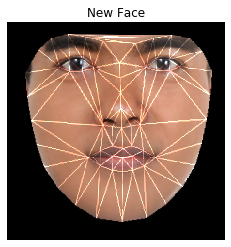
\includegraphics{meta/output_36_0.png}
	\caption{Link the warped triangles together}
\end{figure}

\paragraph{Replace the face on the destination image}\label{header-n166}

\begin{quote}
	The face is ready to be replaced. We cut out the face of the destination
	picture to allow space for the new one.
	
	So we're going to take a new picture, and a destination image without a
	name, and we're going to connect it together.
\end{quote}

\begin{Shaded}
\small
\begin{Highlighting}[]
\NormalTok{img2_face_mask }\OperatorTok{=}\OperatorTok{\textbackslash{}}
\NormalTok{}\NormalTok{ np.zeros_like(img2_gray)}
\NormalTok{img2_head_mask }\OperatorTok{=}\NormalTok{ cv2.fillConvexPoly}\OperatorTok{\textbackslash{}}
\NormalTok{(img2_face_mask, convexhull2, }\DecValTok{255}\NormalTok{)}
\NormalTok{img2_face_mask }\OperatorTok{=}\OperatorTok{\textbackslash{}}
\NormalTok{}\NormalTok{ cv2.bitwise_not(img2_head_mask)}
\NormalTok{img2_head_noface }\OperatorTok{=}\OperatorTok{\textbackslash{}}
\NormalTok{}\NormalTok{ cv2.bitwise_and(img2, img2, mask}\OperatorTok{=}\OperatorTok{\textbackslash{}}
\NormalTok{}\NormalTok{img2_face_mask)}
\NormalTok{result }\OperatorTok{=}\NormalTok{ cv2.add(img2_head_noface,}\OperatorTok{\textbackslash{}}
\NormalTok{ img2_new_face)}
\end{Highlighting}
\end{Shaded}

\begin{figure}
	\centering
	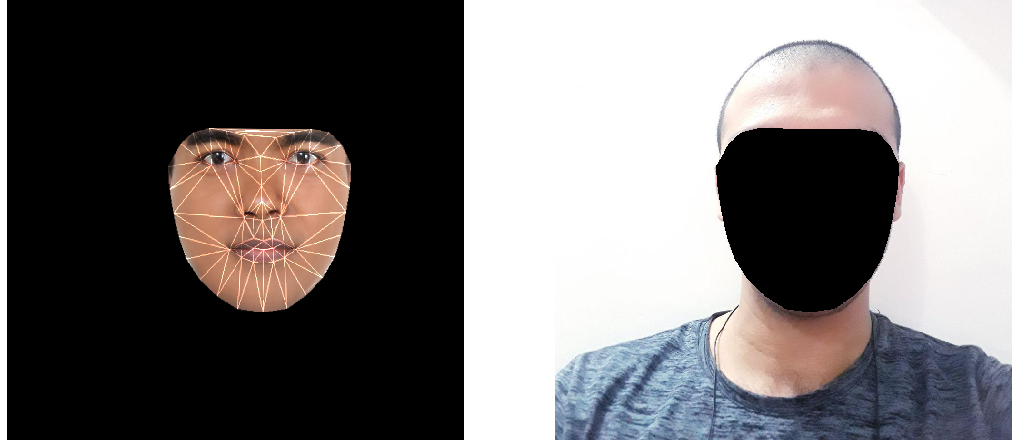
\includegraphics{meta/output_37_0.png}
	\caption{Replace the face on the destination image}
\end{figure}

\paragraph{Seamless Cloning}\label{header-n169}

\begin{quote}
	Finally, the faces are adjusted appropriately and it's time to switch
	the colors such that the source picture matches the destination picture.
	
	We have a built-in feature named "seamlessClone" on Opencv that does
	this process automatically.\\
	We need to take a new picture, take an original destination pic, and a
	mask to cut out the nose, we need to get the middle of the picture, and
	we're ready to go.
\end{quote}

\begin{Shaded}
	\small
	\begin{Highlighting}[]
\NormalTok{(x, y, w, h) }\OperatorTok{= }\OperatorTok{\textbackslash{}}
\NormalTok{  cv2.boundingRect(convexhull2)}
\NormalTok{center_face2 }\OperatorTok{=}\NormalTok{ (}\BuiltInTok{int}\NormalTok{((x }\OperatorTok{+}\NormalTok{ x }\OperatorTok{+}\NormalTok{ w) }\OperatorTok{/ }\OperatorTok{\textbackslash{}}
\NormalTok{ } \DecValTok{2}\NormalTok{), }\BuiltInTok{int}\NormalTok{((y }\OperatorTok{+}\NormalTok{ y }\OperatorTok{+}\NormalTok{ h) }\OperatorTok{/} \DecValTok{2}\NormalTok{))}
\NormalTok{seamlessclone }\OperatorTok{= }\OperatorTok{\textbackslash{}}
\NormalTok{ }\NormalTok{cv2.seamlessClone(result, img2,  }\OperatorTok{\textbackslash{}}
\NormalTok{img2_head_mask, }\OperatorTok{\textbackslash{}}
\NormalTok{center_face2, }\OperatorTok{\textbackslash{}}\NormalTok{cv2.MIXED_CLONE)}
	\end{Highlighting}
\end{Shaded}

\begin{figure}
	\centering
	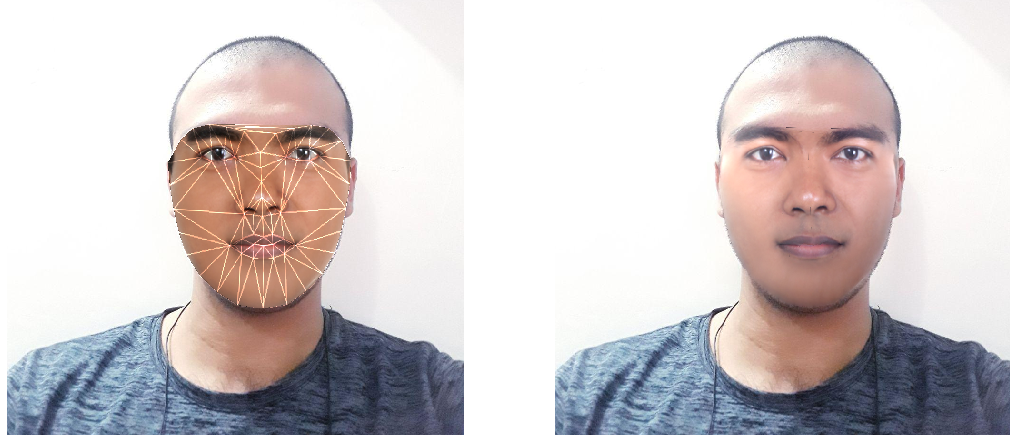
\includegraphics{meta/output_38_0.png}
	\caption{Seamless Cloning}
\end{figure}

\subsection{Future Improvement}\label{header-n357}

This project can be improved by adding some extra features on it like
voice cloning which is is a highly desired feature for personalized
speech interfaces. By adding this feature and improving the existing one
we can even change filming industry. Of course, there were, are, and
will be lots of problems with voice and frame quality as well as there
is one big problem concerned with pattern and the way we speak is hardly
possible to be cloned and imitated. That's way it is interesting to
continue this project. For future improvements, please follow me on
\href{https://github.com/KhasanovR/}{github.com}.

\subsection{Reference }\label{header-n358}

\begin{itemize}
	\item
	Brandon Amos, Jan Harkes, Padmanabhan Pillai, Khalid Elgazzar,\\
	and Mahadev Satyanarayanan.\\
	OpenFace: Face Recognition with Deep Neural Networks.\\
	\url{http://github.com/cmusatyalab/openface}.\\
	Accessed: 2015-11-11
\end{itemize}

\begin{itemize}
	\item
	Levin, Anat, et al. "Seamless image stitching in the gradient domain."
	Computer Vision-ECCV 2004. Springer Berlin Heidelberg, 2004. 377-389.
	\item
	Avidan, S., and Shamir, A. 2007. Seam carving for contentaware image
	resizing. \emph{ACM Transactions on Graphics 26}.
\end{itemize}

\begin{itemize}
	\item
	ACM SIGGRAPH 2008 papers. Association for Computing Machinery, New
	York, NY, USA.
\end{itemize}

\end{document}